In order to correctly predict ACL injuries in real time, data must be collected at a certain frequency so that subtle movements and accelerations are captured in the data. When the sensors were first integrated with the mBed, the rate at which data could be read was not fast enough. Therefore, problems in the library being used were identified and rectified.

Another problem with the performance was the network latency. At first, the data was being transmitted over the network in discrete packets, each several seconds apart. It was determined that the wifi module was buffering the data until a large enough packet was received before transmitting the packet. This was mitigated by configuring the wifi module to send data after each receipt of a data packet. However, the transmission rate still was not fast enough, which required the shortening of the data string used to communicate each data point.

The improvements in data sampling and network transmission rates can be seen in figure~\ref{fig:graph}.

\begin{figure}[h]
  \begin{center}
    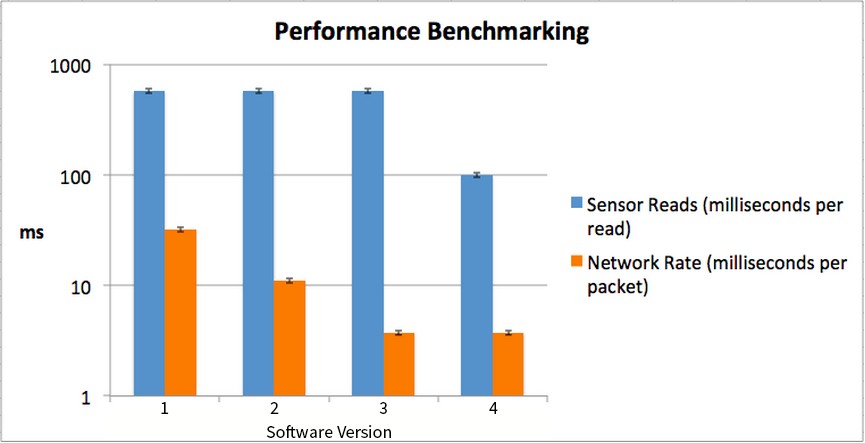
\includegraphics[width=3in]{images/graph.png}
  \end{center}
  \caption{Benchmarking of eKwip}
  \label{fig:graph}
\end{figure}
